\section{related works}

\begin{figure}[t]
    \centering
    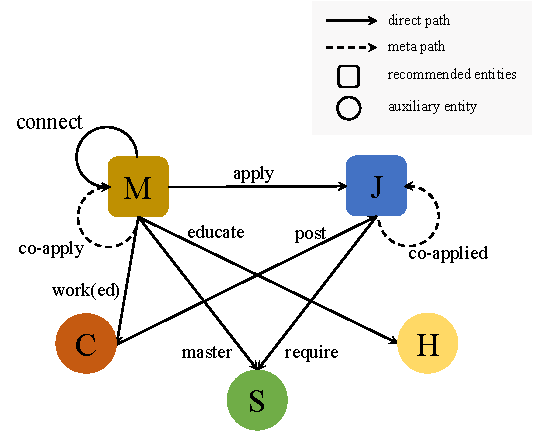
\includegraphics[width=0.6\linewidth]{fig/metagraph.pdf}
    \caption{The metagraph of Workplace Heterogeneous Information Network. It encompasses not only members (M) and jobs (J), which are crucial for Person-Job Fit, but also entities such as skills (S), companies (C), and schools (H).}
    \label{fig:metagraph}
\end{figure}

The related work of our study can be grouped into two main categories, namely,  \textit{Person-Job Fit} and \textit{Heterogeneous Information Network-based Recommendation}.

\subsection{Person-Job Fit}

As a core function of the online recruitment platform, Person-Job Fit \cite{malinowski2006matching} has received widespread attention.

Mainstream works view Person-Job Fit as a text-matching problem between member profiles and job descriptions to fully use the rich contextual knowledge. For example, JLMIA \cite{shen2018joint} is a latent variable model to model job descriptions and member profiles jointly. PJFNN \cite{zhu2018person} encodes member profiles and job descriptions by hierarchical CNN. BPJFNN \cite{qin2018enhancing} leverage BiLSTM to get the semantic representation of each word in member profiles and job descriptions. APJFNN \cite{qin2018enhancing} automatically weighs abilities mentioned in textual information based on historical recruitment results. A transferable deep global match network \cite{bian2019domain} is proposed to solve the domain adaptation problem in three levels for Person-Job Fit. JRMPM \cite{yan2019interview} proposes a matching network with preference modeled to explore the latent preference given the history of the matching process.

\begin{figure*}[!ht]
    \centering
    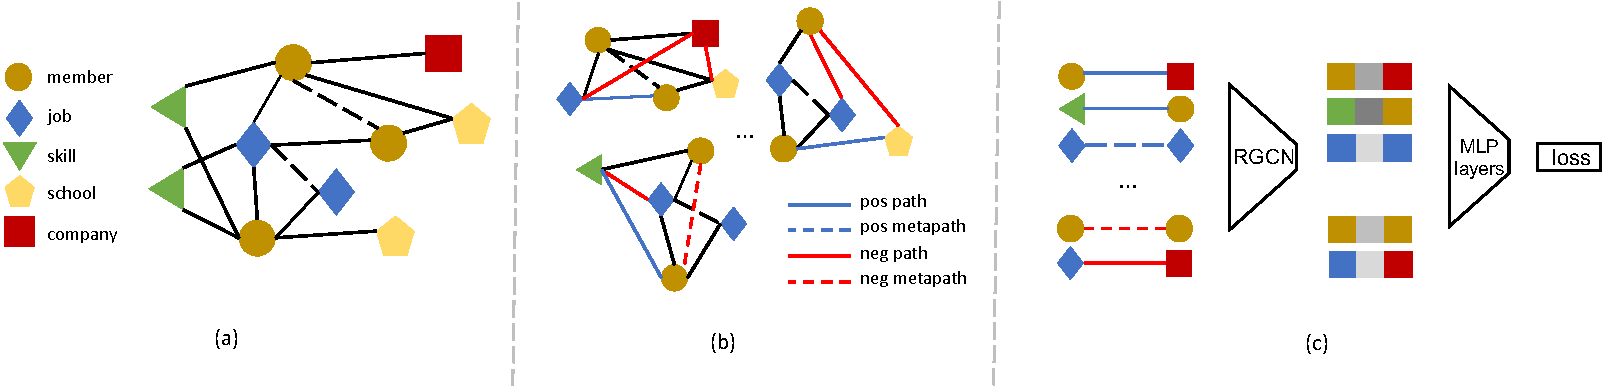
\includegraphics[width=0.75\textwidth]{fig/WHIN_pretrain.pdf}
    \caption{Steps of WHIN pre-training. (a) Workplace heterogeneous graph with metapath. (b) Subgraph sampling for mini-batch pre-training. (c) A pre-training model with encoder-decoder architecture using Link-level pre-training task.}
    \label{fig:WHIN_pretrain}
\end{figure*}

Some works take structure knowledge into consideration. For example, MV-CoN \cite{bian2020learning} adopts a co-teaching mechanism to capture semantic and structure knowledge at the same time. DPGNN \cite{yang2022modeling} explicitly models the two-way selection preference for PJF using GCN. KGRM \cite{yao2022knowledge} model members and jobs as two graphs and fuse prior external knowledge, e.g., skill knowledge graph, into the graph representations.

Previous studies have made good use of textual information, skill entity, and direct interaction between members and jobs to help with Person-Job Fit. However, these studies often overlook the importance of workplace social relations and the incorporation of diverse, heterogeneous knowledge.

\subsection{Heterogeneous Information Network-based Recommendation}

Recommender systems have been widely deployed on the Internet to alleviate information overload \cite{jacoby1984perspectives}. Due to the excellent ability to model complex auxiliary information, Heterogeneous Information Network (i.e., HIN) has become one of the mainstream approaches in recommendation tasks. Depending on the training method, HIN-based models can be divided into \emph{two-stage training-based models} and \emph{end-to-end training-based models} \cite{liu2022survey}.

Two-stage training-based models learn low-dimensional representations of nodes and graph structure using unsupervised tasks and use these representations on various downstream tasks \cite{du2022understanding,bi2022make,huang2023robust,bi2023mm}. Inspired by DeepWalk \cite{perozzi2014deepwalk} and node2Vec \cite{grover2016node2vec}, metapath2vec \cite{dong2017metapath2vec} leverages metapath-based random walks to construct a heterogeneous neighborhood of nodes and leverages skip-gram model to generate node representations. Similarly, HIN2Vec \cite{fu2017hin2vec} defines an unsupervised metapath prediction task and jointly learns metapath predictors and node representations. Many models are proposed based on the graph representation methods such as those above. For example, HERec generates node sequences with metapath-based random walks, uses node2vec to learn node representations, and completes recommendations by representation similarity. MAGNN \cite{fu2020magnn} leverages node content features and information of intermediate nodes along the metapath by node content transformation, intra- and inter-metapath aggregation. Besides, there are some methods not relying on manual metapath, such as HRLHG \cite{jiang2018cross}, NREP \cite{yang2019citation}, and ECHCDR \cite{li2020heterogeneous}.

Compared with two-stage training-based models, end-to-end-based models can use supervision signals directly while training. Thus, they are more customized to specific downstream tasks. For HINs with rich relations, relation-aware graph neural networks can achieve great results. For example, RGCN \cite{schlichtkrull2018modeling} assigns a weight matrix to each type of relation, thus extending GCN \cite{welling2016semi} to multi-relation graphs. DisenHAN \cite{wang2020disenhan} projects nodes into different subspaces using type-specific transformation and uses intra- and inter-aggregation to learn node representations. HAN \cite{wang2019heterogeneous} uses a dual attention mechanism to aggregate information from different metapaths. HPN \cite{ji2021heterogeneous} designs a semantic fusion mechanism for learning the importance of metapath and fusing them judiciously. By using only its immediate connections as input, HGT \cite{hu2020heterogeneous} can learn and extract relevant metapaths for various tasks through its automatic and implicit attention mechanism without requiring manual metapath design.

In this paper, we adopt the two-stage training-based paradigm. During the pre-training stage, we integrate heterogeneous knowledge specific to the Person-Job Fit scenario to obtain diverse entity representations that encompass both structural and textual information. In the downstream stage, we design a novel model that leverages the information from the pre-training stage to filter out noise within professional networks. As a point of comparison, we have also selected two end-to-end-based models as baselines.